% !TEX root = ../../main.tex

\subsection{An in-depth analysis of the NGA mechanism}%
\label{dut:indepth}

As it has been shown in the previous section, there are 
several avenues to achieve tuning of NGA in the DUT-49 framework.
However, a fundamental understanding of the factors and 
energetics of the process itself may
lend itself to prediction of when the phenomenon occurs without 
experimental input, and even lead to the rational design of 
similar materials.

To this end, the adsorption of multiple probes was investigated 
at \SI{77}{\kelvin} with \textit{in situ} continuous low 
temperature microcalorimetry,
in order to observe the influence of the guest on the mechanism of
adsorption and NGA. To obtain a baseline of adsorption in 
the \textit{op} phase, a non-flexible alternative is used. 
DUT-149 is the most similar material out of all previously studied
analogues, as it has the same linker length and nearly identical pore
size and surface area.

Four gas probes were used, chosen as they 
have a non-trivial saturation pressure at this temperature: Ar,
\ce{N2}, \ce{CO} and \ce{O2}. Argon, as a 
noble gas, has a completely spherical molecule, which does not 
have any specific host-guest or guest-guest interactions. Nitrogen
is commonly used as the probe in material characterisation, 
and carries a weak quadrupole. Carbon monoxide has been used 
as it often forms coordination bonds through electron donation,
as well as being a weak dipole and quadrupole.
Finally oxygen has a weaker quadrupolar moment than 
nitrogen, and can interact with the surface in a similar way.
It is worth noting that both argon and carbon monoxide are below 
their freezing point at this temperature. A table with 
relevant properties of the probes used at the experimental
conditions can be found in \autoref{appx:dut:probes}.

\subsubsection{Results and initial observations}

A large dataset was gathered
on these materials as experiments were performed with different 
amounts of sample, different gas introduction flowrates, as well as repeats
with identical conditions to ensure that factors such as 
equilibrium or diffusion do not play a role in the results. 
No desorption isotherms can be recorded using this method, with
leads to an inability to obtain an enthalpy curve corresponding 
to the \textit{cp} form at low pressure. A list 
of experiments, as well as all isotherms and enthalpy curves measured can
be found in \autoref{appx:dut}.

\begin{figure}[p]
    \centering
    
    \begin{subfigure}{0.43\linewidth}
        \includegraphics[width=\linewidth]{ltc/dut-49-CO-log}%
        % \caption{}\label{dut:fgr:dut-48-prop-log}
    \end{subfigure}%
    \begin{subfigure}{0.43\linewidth}
        \includegraphics[width=\linewidth]{ltc/dut-149-CO-log}%
        % \caption{}\label{dut:fgr:dut-48-prop-enth}
    \end{subfigure}%

    \begin{subfigure}{0.43\linewidth}
        \includegraphics[width=\linewidth]{ltc/dut-49-CO-enth}%
        % \caption{}\label{dut:fgr:dut-48-prop-log}
    \end{subfigure}%
    \begin{subfigure}{0.43\linewidth}
        \includegraphics[width=\linewidth]{ltc/dut-149-CO-enth}%
        % \caption{}\label{dut:fgr:dut-48-prop-enth}
    \end{subfigure}%

    \begin{subfigure}{0.43\linewidth}
        \includegraphics[width=\linewidth]{ltc/dut-49-N2-log}%
        % \caption{}\label{dut:fgr:dut-48-prop-log}
    \end{subfigure}%
    \begin{subfigure}{0.43\linewidth}
        \includegraphics[width=\linewidth]{ltc/dut-149-N2-log}%
        % \caption{}\label{dut:fgr:dut-48-prop-enth}
    \end{subfigure}%

    \begin{subfigure}{0.43\linewidth}
        \includegraphics[width=\linewidth]{ltc/dut-49-N2-enth}%
        % \caption{}\label{dut:fgr:dut-48-prop-log}
    \end{subfigure}%
    \begin{subfigure}{0.43\linewidth}
        \includegraphics[width=\linewidth]{ltc/dut-149-N2-enth}%
        % \caption{}\label{dut:fgr:dut-48-prop-enth}
    \end{subfigure}%

    \caption{Carbon monoxide (top) and nitrogen (bottom) isotherms and 
    enthalpy curves measured on DUT-49 (left) and DUT-149 (right).}%
    \label{dut:fgr:dut-ltc-comp1}
\end{figure}

\begin{figure}[p]
    \centering
    
    \begin{subfigure}{0.43\linewidth}
        \includegraphics[width=\linewidth]{ltc/dut-49-Ar-log}%
        % \caption{}\label{dut:fgr:dut-48-prop-log}
    \end{subfigure}%
    \begin{subfigure}{0.43\linewidth}
        \includegraphics[width=\linewidth]{ltc/dut-149-Ar-log}%
        % \caption{}\label{dut:fgr:dut-48-prop-enth}
    \end{subfigure}%

    \begin{subfigure}{0.43\linewidth}
        \includegraphics[width=\linewidth]{ltc/dut-49-Ar-enth}%
        % \caption{}\label{dut:fgr:dut-48-prop-log}
    \end{subfigure}%
    \begin{subfigure}{0.43\linewidth}
        \includegraphics[width=\linewidth]{ltc/dut-149-Ar-enth}%
        % \caption{}\label{dut:fgr:dut-48-prop-enth}
    \end{subfigure}%

    \begin{subfigure}{0.43\linewidth}
        \includegraphics[width=\linewidth]{ltc/dut-49-O2-log}%
        % \caption{}\label{dut:fgr:dut-48-prop-log}
    \end{subfigure}%
    \begin{subfigure}{0.43\linewidth}
        \includegraphics[width=\linewidth]{ltc/dut-149-O2-log}%
        % \caption{}\label{dut:fgr:dut-48-prop-enth}
    \end{subfigure}%
    
    \begin{subfigure}{0.43\linewidth}
        \includegraphics[width=\linewidth]{ltc/dut-49-O2-enth}%
        % \caption{}\label{dut:fgr:dut-48-prop-log}
    \end{subfigure}%
    \begin{subfigure}{0.43\linewidth}
        \includegraphics[width=\linewidth]{ltc/dut-149-O2-enth}%
        % \caption{}\label{dut:fgr:dut-48-prop-enth}
    \end{subfigure}%
    
    \caption{Argon (top) and oxygen (bottom) isotherms and 
    enthalpy curves measured on DUT-49 (left) and DUT-149 (right).}%
    \label{dut:fgr:dut-ltc-comp2}
\end{figure}

Selected isotherms and corresponding enthalpy curves for both 
DUT-49 and DUT-149 are shown in \autoref{dut:fgr:dut-ltc-comp1}
for \ce{N2} and \ce{CO} and in \autoref{dut:fgr:dut-ltc-comp2}
for \ce{Ar} and \ce{O2}. A cursory observation of the isotherms
reveals that the DUT-149 framework is not as stiff as 
previously assumed. A clear NGA step can be found in the 
oxygen isotherm, suggesting that adsorption of this probe is capable 
of overcoming the higher energy barrier of linker buckling in 
this methyl functionalised version.
If comparing the isotherms measured on the two materials, they
are seen to be nearly identical until structural contraction.
The total amount adsorbed after pore re-opening is also in a 
2\% range with all probes. The assumption that the mechanism 
of adsorption in DUT-49 can be likened to its functionalised
version holds in this case.
\todo{Talk about CO}

Another surprising behaviour
can be seen in the nitrogen isotherm on DUT-49. While an NGA
discontinuity is still present, structural re-opening takes
place in several distinct steps, each accompanied by a sharp 
peak in the enthalpy curve. This behaviour in in
agreement with the study published by 
 \citet{krauseEffectCrystalliteSize2018}
on the evolution of the contraction step with variation of 
crystallite size. In their paper, the increase of average 
crystal dimensions is seen to change the material from non-flexible 
to a progressively better defined NGA transition. \textit{In situ} 
PXRD shows that between complete structural stiffness and a 
purely \textit{op}/\textit{cp} phase transition, several intermediate 
pore forms can be accessed. It can therefore be theorised that 
nitrogen adsorption takes place near the lower limit of 
favourable transition energetics, where particulate surface 
effects can have a high influence on the stability domain of
the open pore form.

\subsubsection{Physical state of the adsorbate in the material pores}

As two of the four gas probes are below their respective freezing point
at experimental conditions, a question arises about the state of
the adsorbate in the pores of the material. While a structuring of
the fluid similar to a solid phase is possible inside the 
pores of various adsorbents~\cite{llewellynAdsorptionMFItypeZeolites1993a},
it is often that the adsorbed phase is more similar to a liquid,
even at low temperatures.

\begin{figure}[htb]
    \centering
    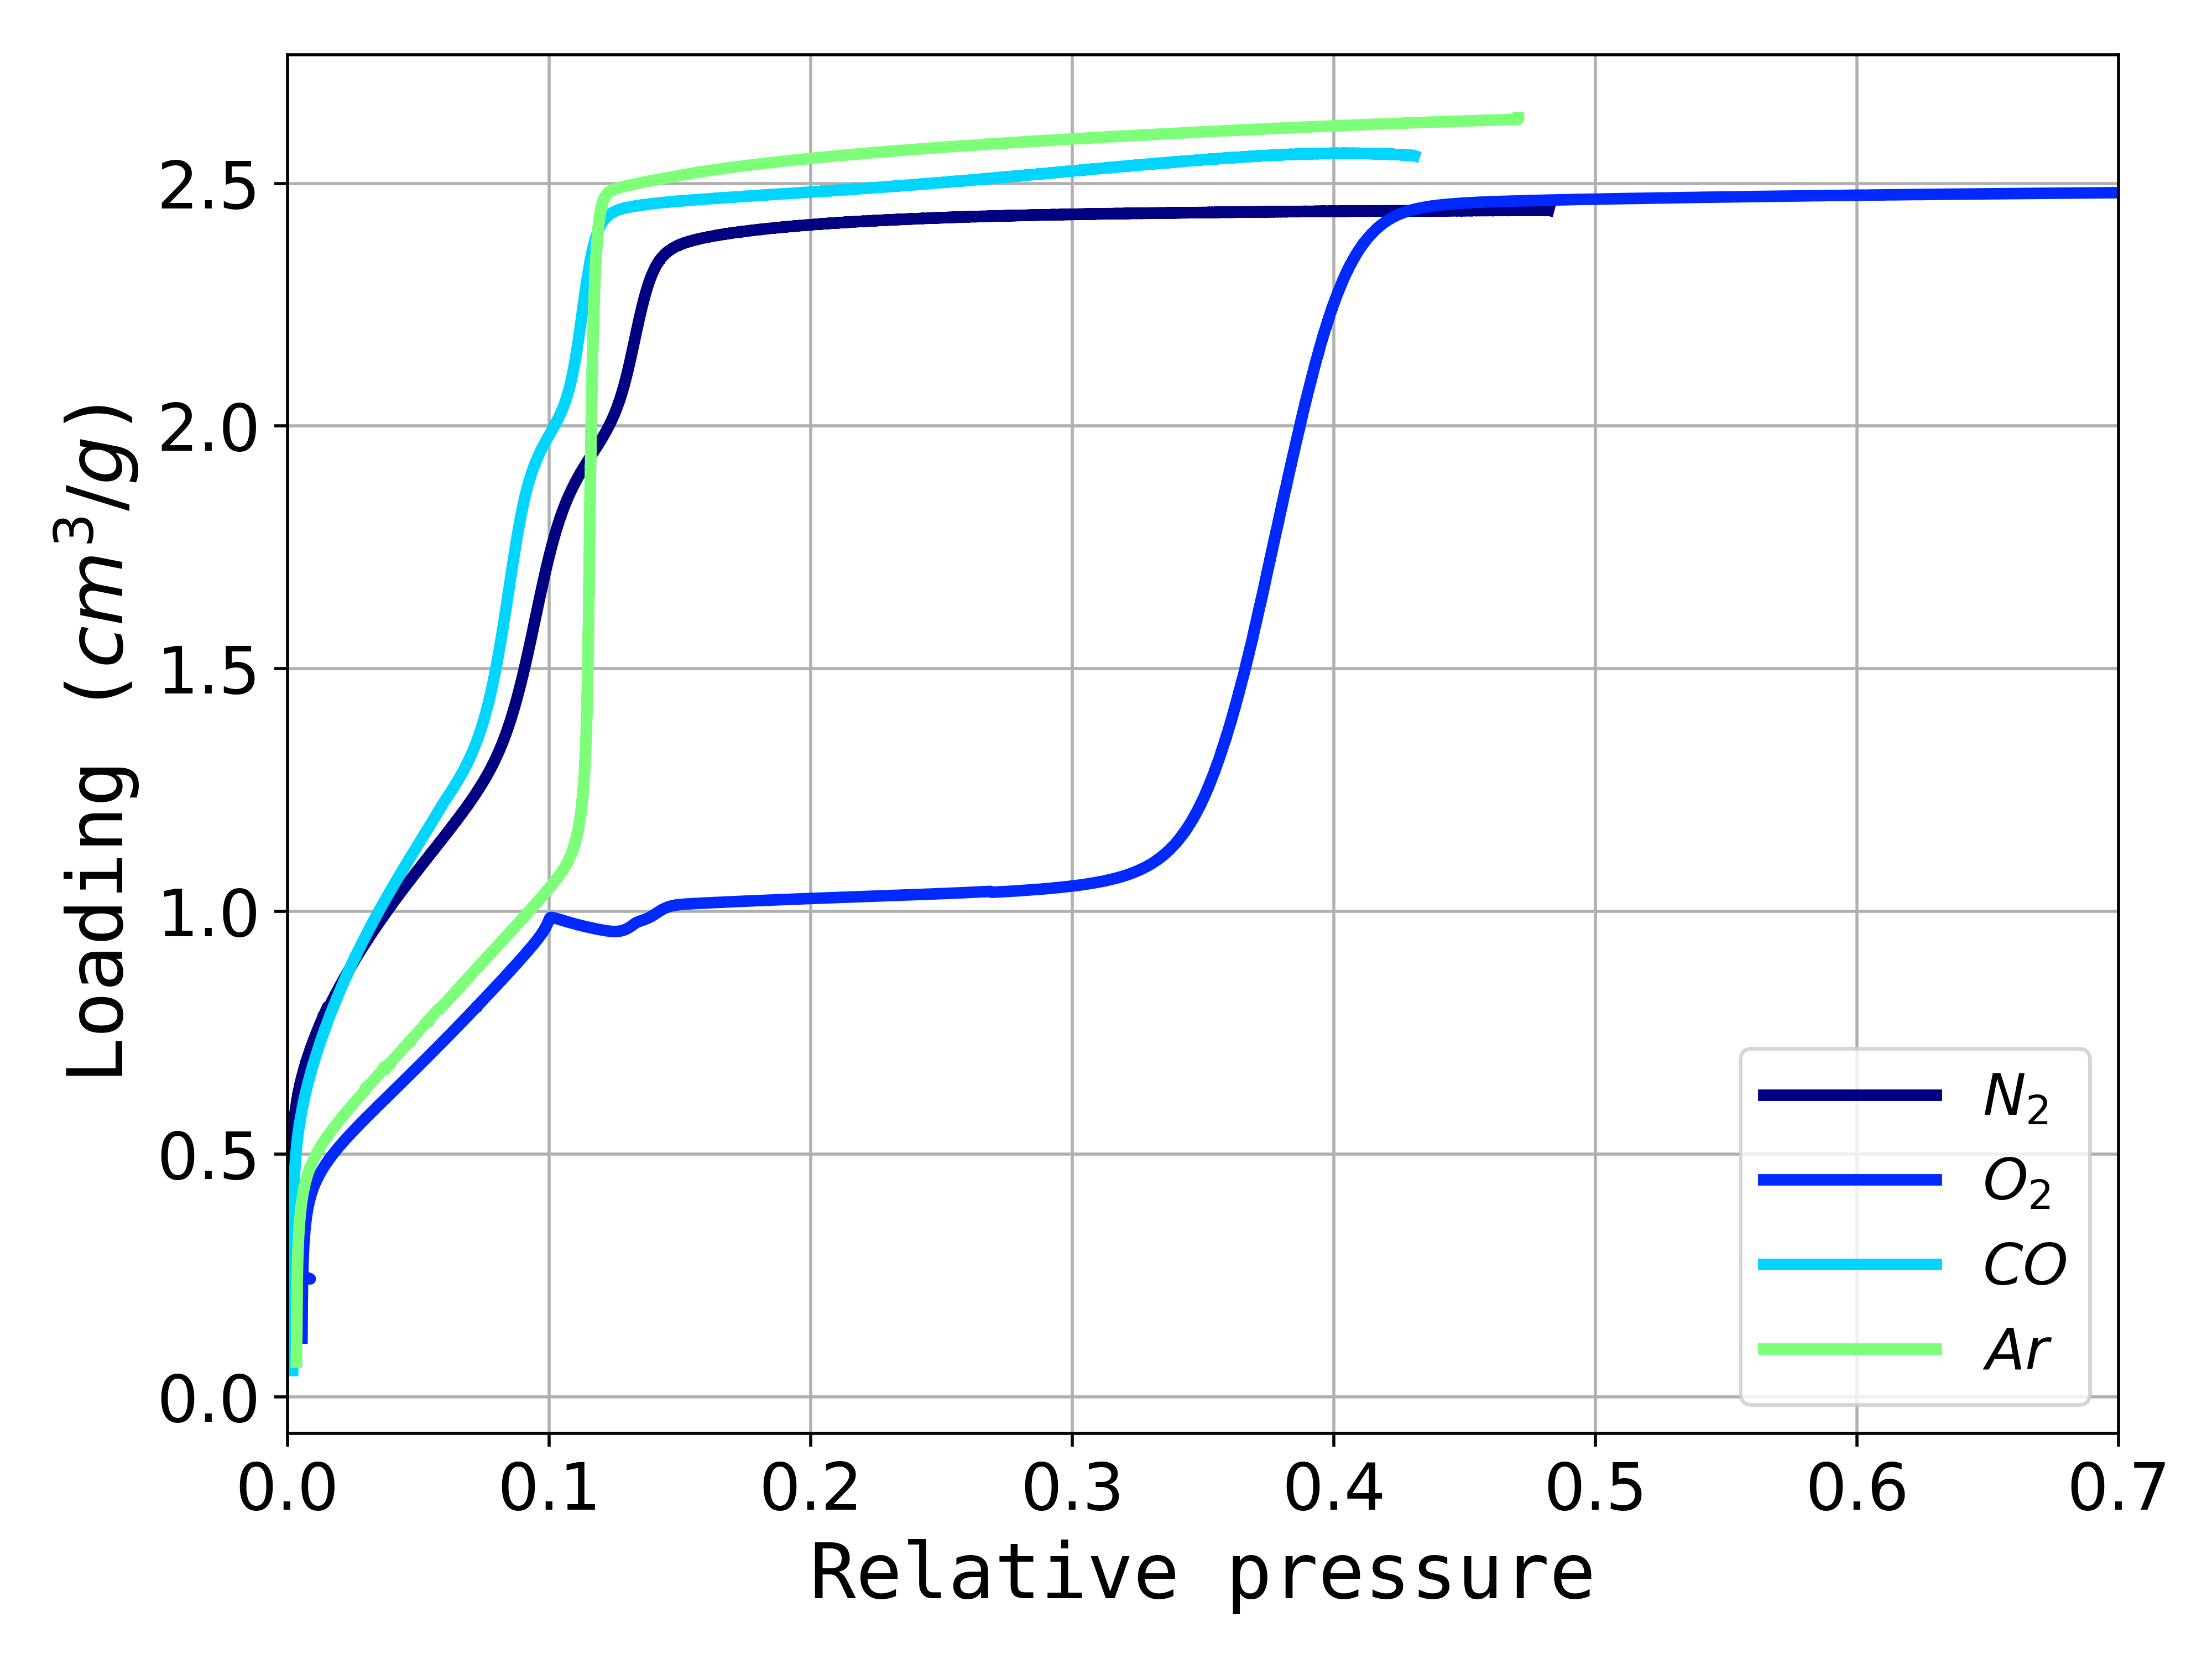
\includegraphics[width=0.5\linewidth]{ltc/DUT-149-volume}%
    \caption{Volumetric adsorption isotherms of all probe gasses
    on DUT-149. The density of the adsorbate was obtained assuming
    from the liquid density at the corresponding temperature.
    It is assumed that the structure re-opening after oxygen
    adsorption is complete.}%
    \label{dut:fgr:dut-volume}
\end{figure}

A simple method to check whether the phase of all measured probes
is close to a liquid state, assuming that the accessible void space 
is identical with all probes, is to convert measured isotherms 
to a fluid volume basis and compare the total pore volume as determined
with each fluid. The density used for this conversion is the 
liquid density of the saturated liquid as calculated using the 
REFPROP equation of state at the isotherm temperature.
\autoref{dut:fgr:dut-volume} plots isotherms measured on DUT-149
transformed using this method. All isotherms reach a plateau at around 
\SI{2.5}{\centi\metre^3\per\gram}, confirming that the fluid in 
the pores can be considered in a liquid state.

\subsubsection{Specific guest-host interactions}

A common feature to almost all measured isotherms on the DUT-49 systems
is the equivalent adsorption mechanism before structural transition 
takes place.
Indeed if enthalpy curves recorded with different adsorbates at different
temperatures below the critical point of the fluid are compared at low 
loading, they may be mistaken for the same datapoints shifted to
various enthalpy values.
In adsorption in the \textit{op} state, this ``typical'' enthalpy 
curve first increases to a local maxima, followed
by a gentle downward slope. The pore filling step (or steps)
are accompanied by an increase in \(\Delta_{ads} \dot{h}\),
an indication of high guest-guest interactions. It is in this 
pore filling step where the structural contraction occurs. 
This prototypical enthalpy profile of the \textit{op} phase 
is also seen on most DUT-49 analogues
in \autoref{dut:comparison}, suggesting that it is a consequence of 
the topology of this structure.
These features suggest that specific interactions with the framework
are generally low. The only 
exception to this case are adsorbates which can interact with the 
Cu paddlewheel, either through adduct formation, 
electron donation or \(\pi\) backbonding interactions. 

\begin{figure}[htb]
    \centering
    \begin{subfigure}[c]{0.5\linewidth}
        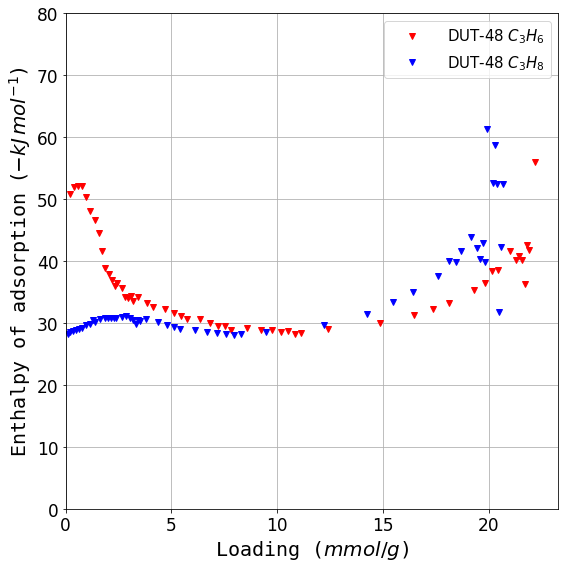
\includegraphics[width=\linewidth]{rtc/dut-48-prop-enth}%
        \caption{}\label{dut:fgr:dut-48-prop-enth}
    \end{subfigure}%
    \begin{subfigure}[h]{0.5\linewidth}
        \centering
        \(\vcenter{\hbox{{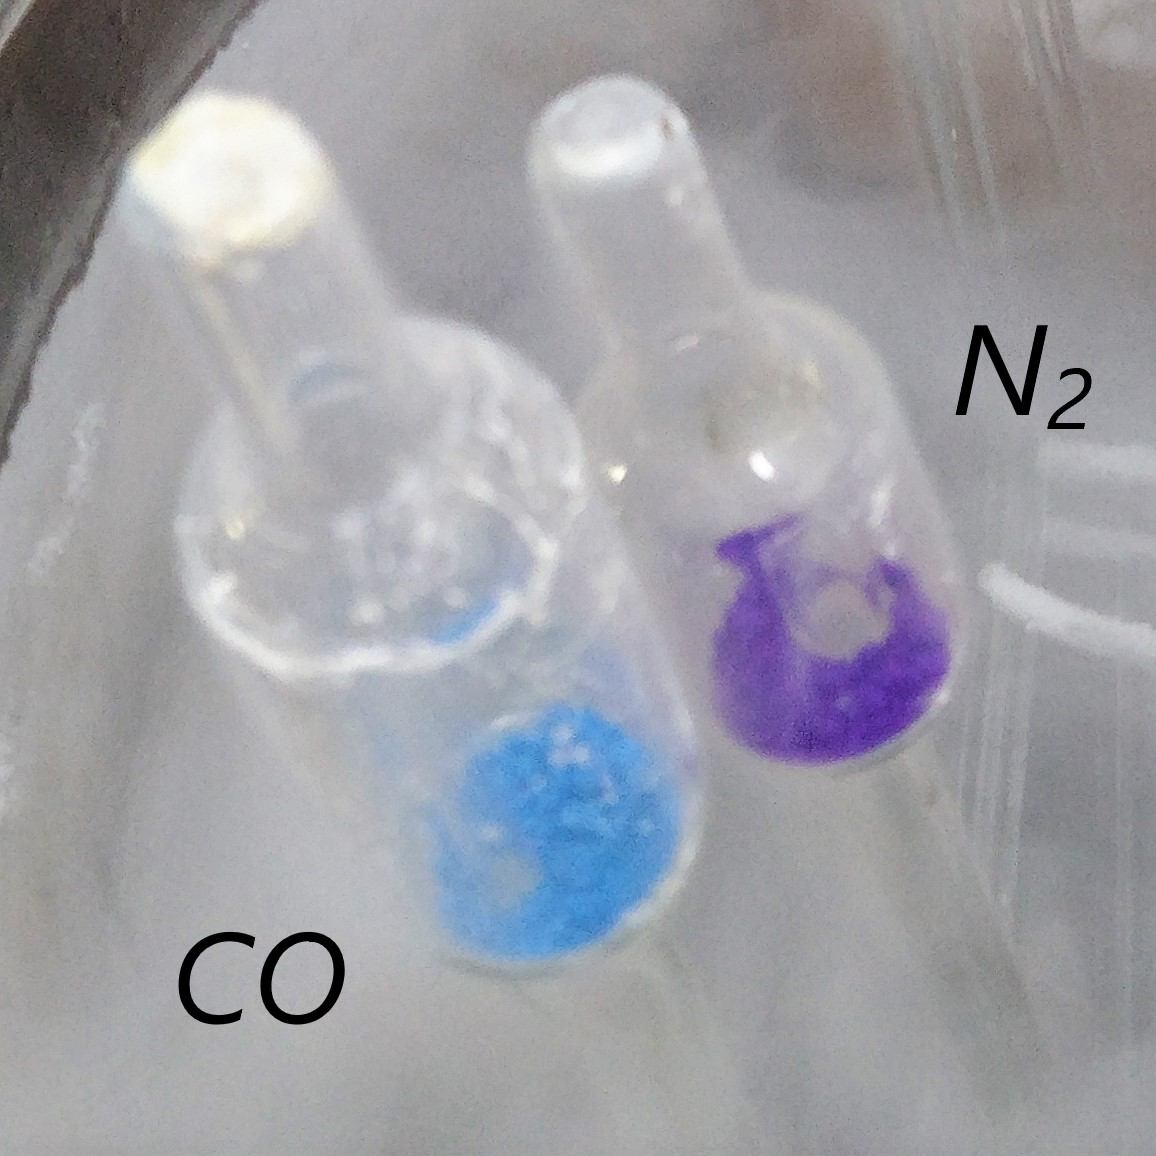
\includegraphics[width=0.9\linewidth]{dut-co}}}}\)%
        \caption{}\label{dut:fgr:dut-co}
    \end{subfigure}%
    \caption{(a) Enthalpy curves of propane and propylene on DUT-48 as 
    a function of fractional loading, with higher enthalpy of 
    adsorption of the unsaturated hydrocarbon at low loading as an 
    indication of \(\pi\)-Cu interactions. (b) Photo of DUT-149 cells
    filled with CO and \ce{N2} at \SI{77}{\kelvin}. Note the 
    colour change of the CO-filled cell as evidence of the formation of 
    \ce{Cu(II)\bond{...}CO} adducts.}%
    \label{dut:fgr:dut-48-prop}
\end{figure}

Such effects are noticeable in the CO adsorption isotherms, 
as the initial measured differential enthalpy of adsorption is around 
\SI{40}{\kilo\joule\per\mol}, consistent with the formation of 
\ce{Cu(II)\bond{...}CO} adducts as seen in similar paddlewheel based 
MOF such as HKUST-1~\cite{prestipinoLocalStructureFramework2006}. 
Indeed, a visual examination of the carbon monoxide saturated 
DUT-149 at \SI{77}{\kelvin} 
(\autoref{dut:fgr:dut-co}) shows a pronounced colour shift and 
suggests a change in the coordination sphere of the copper 
atoms. As the sample is brought to ambient temperature, the 
cyan colour disappears, attesting that there is no strong 
coordination bond, such as is typical in more stable 
\ce{Cu(I)\bond{...}CO} coordination compounds.

A separate study on the possible interaction of 
\(\pi\) bond containing unsaturated hydrocarbons was performed
using ambient temperature calorimetry. Propane and propylene 
isotherms and enthalpy curves were recorded on the shorter 
linker, non-flexible DUT-48. \autoref{dut:fgr:dut-48-prop-enth}
reveals that there is indeed a larger enthalpy of adsorption
at low loadings when propylene is used as the probe gas, with 
the curves overlapping after the initial region. The difference 
of around \SI{20}{\kilo\joule\per\mol} between the two initial
enthalpies of adsorption is consistent to what has been predicted
and recorded on the copper center in 
HKUST-1~\cite{rubesAdsorptionPropanePropylene2013}, and can
be explained through the formation of a partial dative bond
between the propylene \(\pi\) orbital and the \ce{Cu^{2+}}
cation. 

In both the case of CO and \ce{C3H6}, the 
stronger interactions occur only at fractional loadings lower
than 0.1, before the occurrence of NGA. The enthalpy of 
adsorption after this region take values which are close to
those of similar probes (\ce{CO}-\ce{N2}, \ce{C3H6}-\ce{C3H8}).
This is further evidence that, while specific guest-host interactions
may exist, they play little to no role in the mechanism of contraction.

\subsubsection{Pore filling mechanism of the \textit{op} phase}

If focusing on the pore filling behaviour of DUT-149, two types
of mechanisms can be seen. While the initial part of the isotherm 
(below \(0.1~p/p_0\)) is typical of BET-type multilayer adsorption
with a possible micropore filling step at very low pressure,
the large framework pores are seen to be filled in either a single or
two-step process.
Both nitrogen and carbon monoxide have two distinct filling
steps, corresponding to the octahedral and tetrahedral pores,
respectively. The two steps are accompanied by identical 
peaks in the enthalpy curve. This points to a highly similar 
filling process for both pores, with cooperative adsorption
dominating the pore filling mechanism rather than guest-host 
effects. The argon isotherm, similar to the behaviour of 
butane at \SI{303}{\kelvin}, shows a very sharp single-step process,
which can be likened to condensation in a mesopore. As the 
two pores in the DUT-49/149 framework are interconnected through 
windows of \(\approx\)\SI{1}{\nano\metre}, pore filling 
in one type of pore can induce filling in the adjacent pore of 
a larger size. The sudden transition to the fluid phase can further
be understood if considering the MOF pores are nearly in the mesoscale 
range. Adsorption in such pores can be characterised through 
the formation of a vapour-like spinodal if the pore size is within
a ``critical hysteresis radius''~\cite{hiratsukaCriticalEnergyBarrier2016},
a metastable state which subsequently undergoes a phase change when
nucleation occurs. Unfortunately, the presence of a hysteresis curve
cannot be confirmed, as no desorption isotherms can be obtained 
through the continuous method.

\begin{wrapfigure}{h}{0.3\textwidth}
	\centering
	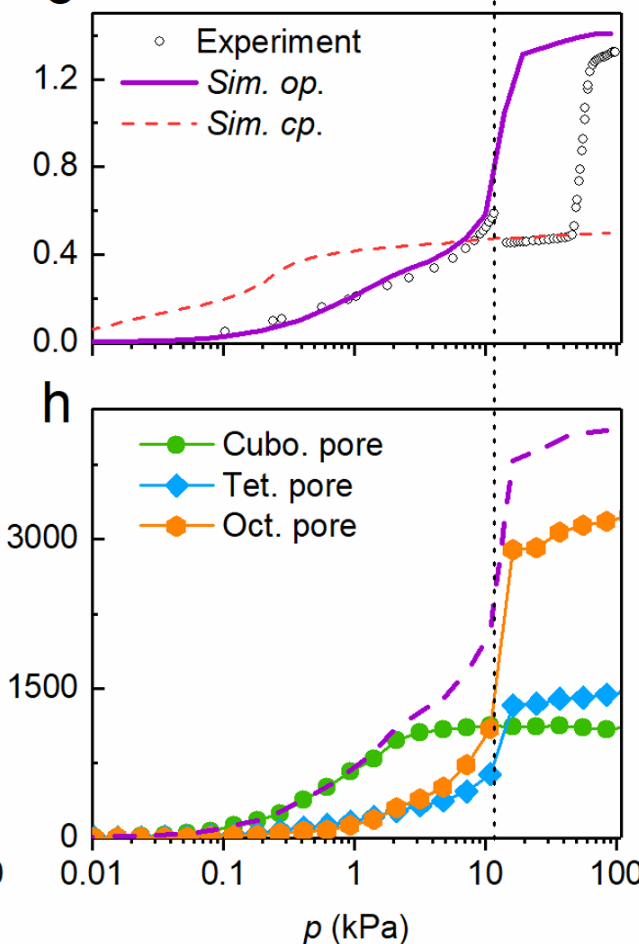
\includegraphics[width=0.27\textwidth]{pore-filling}%
    \caption{A dissection of the \ce{CD4} isotherm
    at \SI{111}{\kelvin} 
    in components of adsorption in each type of pore.}%
	\label{dut:fgr:pore-filling}
\end{wrapfigure}
For a better understanding of the pore filling mechanism, adsorption
in DUT-49 was studied through \textit{in situ} neutron powder diffraction
(NPD) during adsorption of deuterated methane \ce{CD4} at \SI{111}{\kelvin},
and complemented through grand canonical monte carlo (GCMC) simulations
of the same system. Refinement of the NPD patterns allowed the distribution
of the adsorbed \ce{CD4} in a structural unit cell to be obtained, which
was further analysed using a radial distribution function to determine
how the filling of each pore as a function of pressure occurs. 
Results show that adsorption first takes place inside the SBU,
on the copper open metal sites. 
\autoref{dut:fgr:pore-filling} reveals how
the filling of each pore contributes to the overall isotherm.
As expected, the SBU pore is completely filled at very low pressures
and corresponds to the initial ``knee'' in the adsorption isotherm. Gradual
pore filling then takes place until a condensation step which 
leads to complete filling of all pores. This step coincides with 
the structural transition associated with NGA and is likely a driver 
for the contraction.
\todo{need data from Simon for figure...}

\subsubsection{Relating adsorption conditions to structural contraction}

As continuous adsorption introduction is a time-resolved technique, 
the signal obtained during the structural contraction step can 
be examined for clues about the energetics of transition. An example 
of peaks obtained during the NGA step can be observed in 
\autoref{dut:fgr:ltc-peaks}. It is immediately obvious that 
the nitrogen transition is actually endothermic, unlike the 
signal obtained during the argon and oxygen experiments.

\begin{figure}[htb]
    \centering
    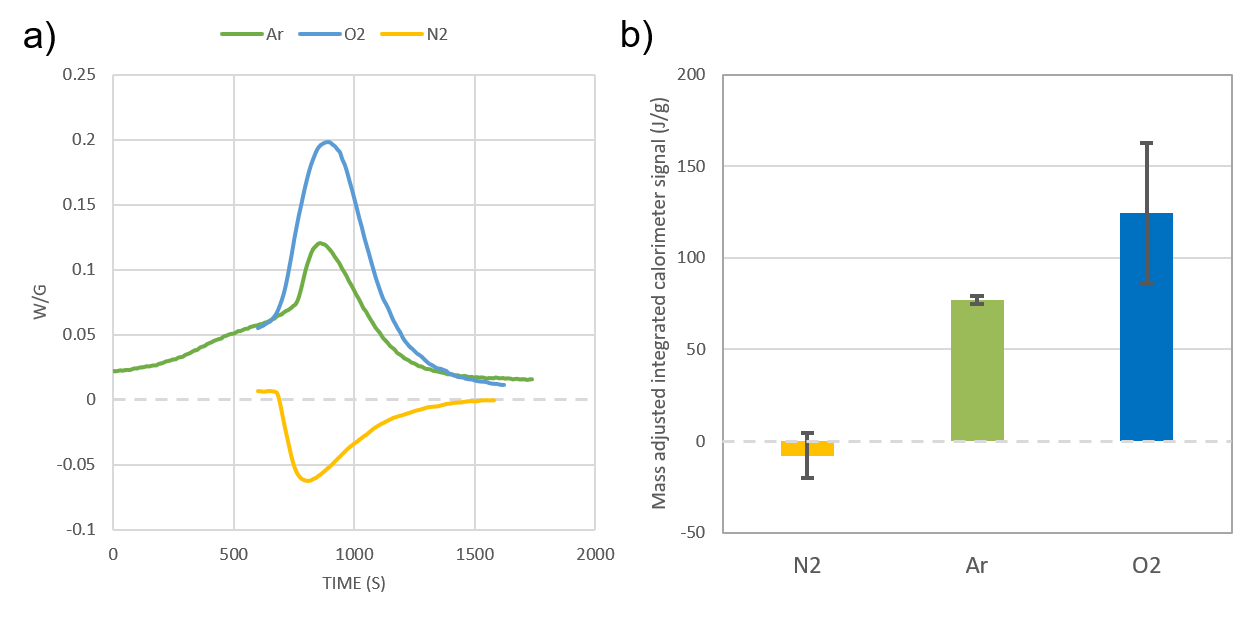
\includegraphics[width=0.8\linewidth]{ltc-peaks}%
    \caption{(a) An example of three recorded signals during 
    structural contraction on DUT-49 with nitrogen, argon and 
    oxygen. (b) Integrated calorimetric heat signal from 
    nitrogen, argon and oxygen experiments. Error bars 
    represent one standard deviation from the dataset mean.}%
    \label{dut:fgr:ltc-peaks}
\end{figure}

As the system contraction is responsible for a pressure increase
in the unit cell, transition of any crystallite is likely to be a
trigger of a cascade effect, where local increases in guest partial 
pressure induce collapse of neighbouring particles. As such,
deconvolution of the calorimeter peaks during the NGA is a nearly 
impossible task, since minute factors such as diffusion effects,
cell geometry, sample amount or flowrate can drastically change 
the shape of the evolved signal. However, integrating the heat 
recorded throughout the NGA step should give an independent value of such
substeps as it represents the total heat of the transition. 
The average values of the observed energetics of 
NGA presented in \autoref{dut:fgr:ltc-peaks} paints an interesting
picture regarding the influence of the adsorbate.
The stress induced by the probe gas differs with its physical
nature. A good indication of guest-guest interactions at 
a particular temperature is the enthalpy of vaporisation 
(\(\Delta H_{vap}\)) of a saturated liquid. Indeed, the magnitude
of the transition energy appears to be related to this value, as
oxygen which has the highest \(\Delta H_{vap}\) out of all probes 
used also capable of inducing transition in stiffer frameworks. By
plotting the enthalpy of vaporisation for different adsorbates
and adjusting it by assuming the energetic barrier is purely 
entropic, a remarkable correlation with the existence windows
of NGA extending up to ambient temperature and with different probes
can be found, as seen in \autoref{dut:fgr:hvap-model}.
This empiric model can seemingly predict the energetic limit
for a favourable transition, and is likely a reflection of the 
true energetics of the system in the subset of cases where the 
assumption of pure guest-guest interaction overcoming an entropic
barrier holds. However, carbon monoxide is seen to deviate from
the predicted behaviour and exhibit no NGA at \SI{77}{\kelvin}. 
It is likely that the increased interactions with the framework metal
sites account for a larger energy barrier.

\begin{figure}[htb]
    \centering
    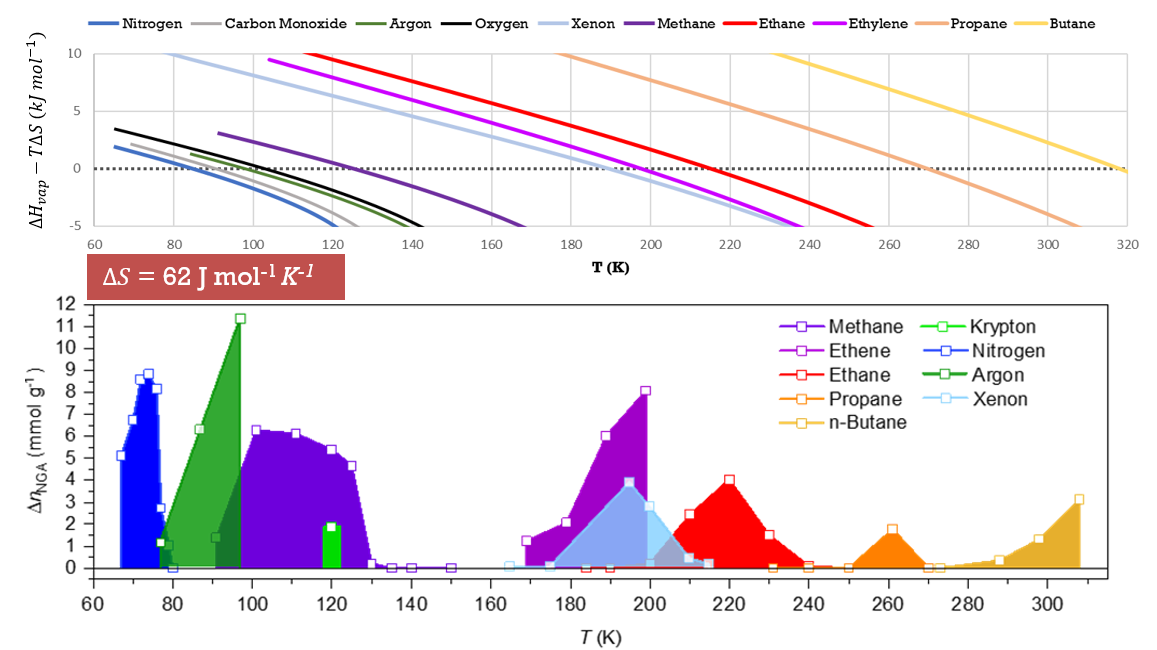
\includegraphics[width=0.9\linewidth]{hvap-model}%
    \caption{A surface obtained by subtracting an entropic 
    contribution from the enthalpy of vaporisation of 
    several common adsorbates (top) compared to the 
    magnitude and existence region of NGA measured on 
    DUT-49 with various adsorbates.}%
    \label{dut:fgr:hvap-model}
\end{figure}

It is also worth noting that an inverse relationship exists 
between the exothermicity of the transition step and the 
amount of fluid ejected from the structure pores during the NGA 
step, with nitrogen experiments generating the highest \(\Delta n_{NGA}\)
even if the transition to a \textit{cp} state is incomplete.
As the energy required for the expulsion of the material from the 
pores can be thought of as the enthalpy of desorption of the same amount
from the closed pore, this component should be considered if 
attempting to calculate the energy difference between the two states.
Repeating continuous microcalorimetry experiments at a different 
temperature, such as in an argon bath at \SI{87}{\kelvin}, would 
allow for the temperature dependence of the adsorbate influence 
to be recorded. It is highly likely that NGA would be completely 
suppressed in the case of nitrogen and perhaps argon on DUT-49.

\subsubsection{Effect of cycling on DUT-49 transition}

By increasing the partial pressure of any of the low temperature 
calorimetry probes over \(\approx 0.8~p/p_0\), a re-opening
of the structure can be observed. If the sample is exposed to 
vacuum while at \SI{77}{\kelvin}, it collapses to the \textit{cp}
phase during desorption and undergoes a structural breakdown 
due to the instability of this form. However, if the temperature 
is raised above the adsorbate critical point while maintaining the
sample at saturation pressure, the material can be kept in the 
\textit{op} phase. No NGA has been observed with supercritical 
adsorbates, which is why the material is normally activated through
this method. 

\begin{figure}[htb]
    \centering
    \begin{subfigure}[c]{0.5\linewidth}
        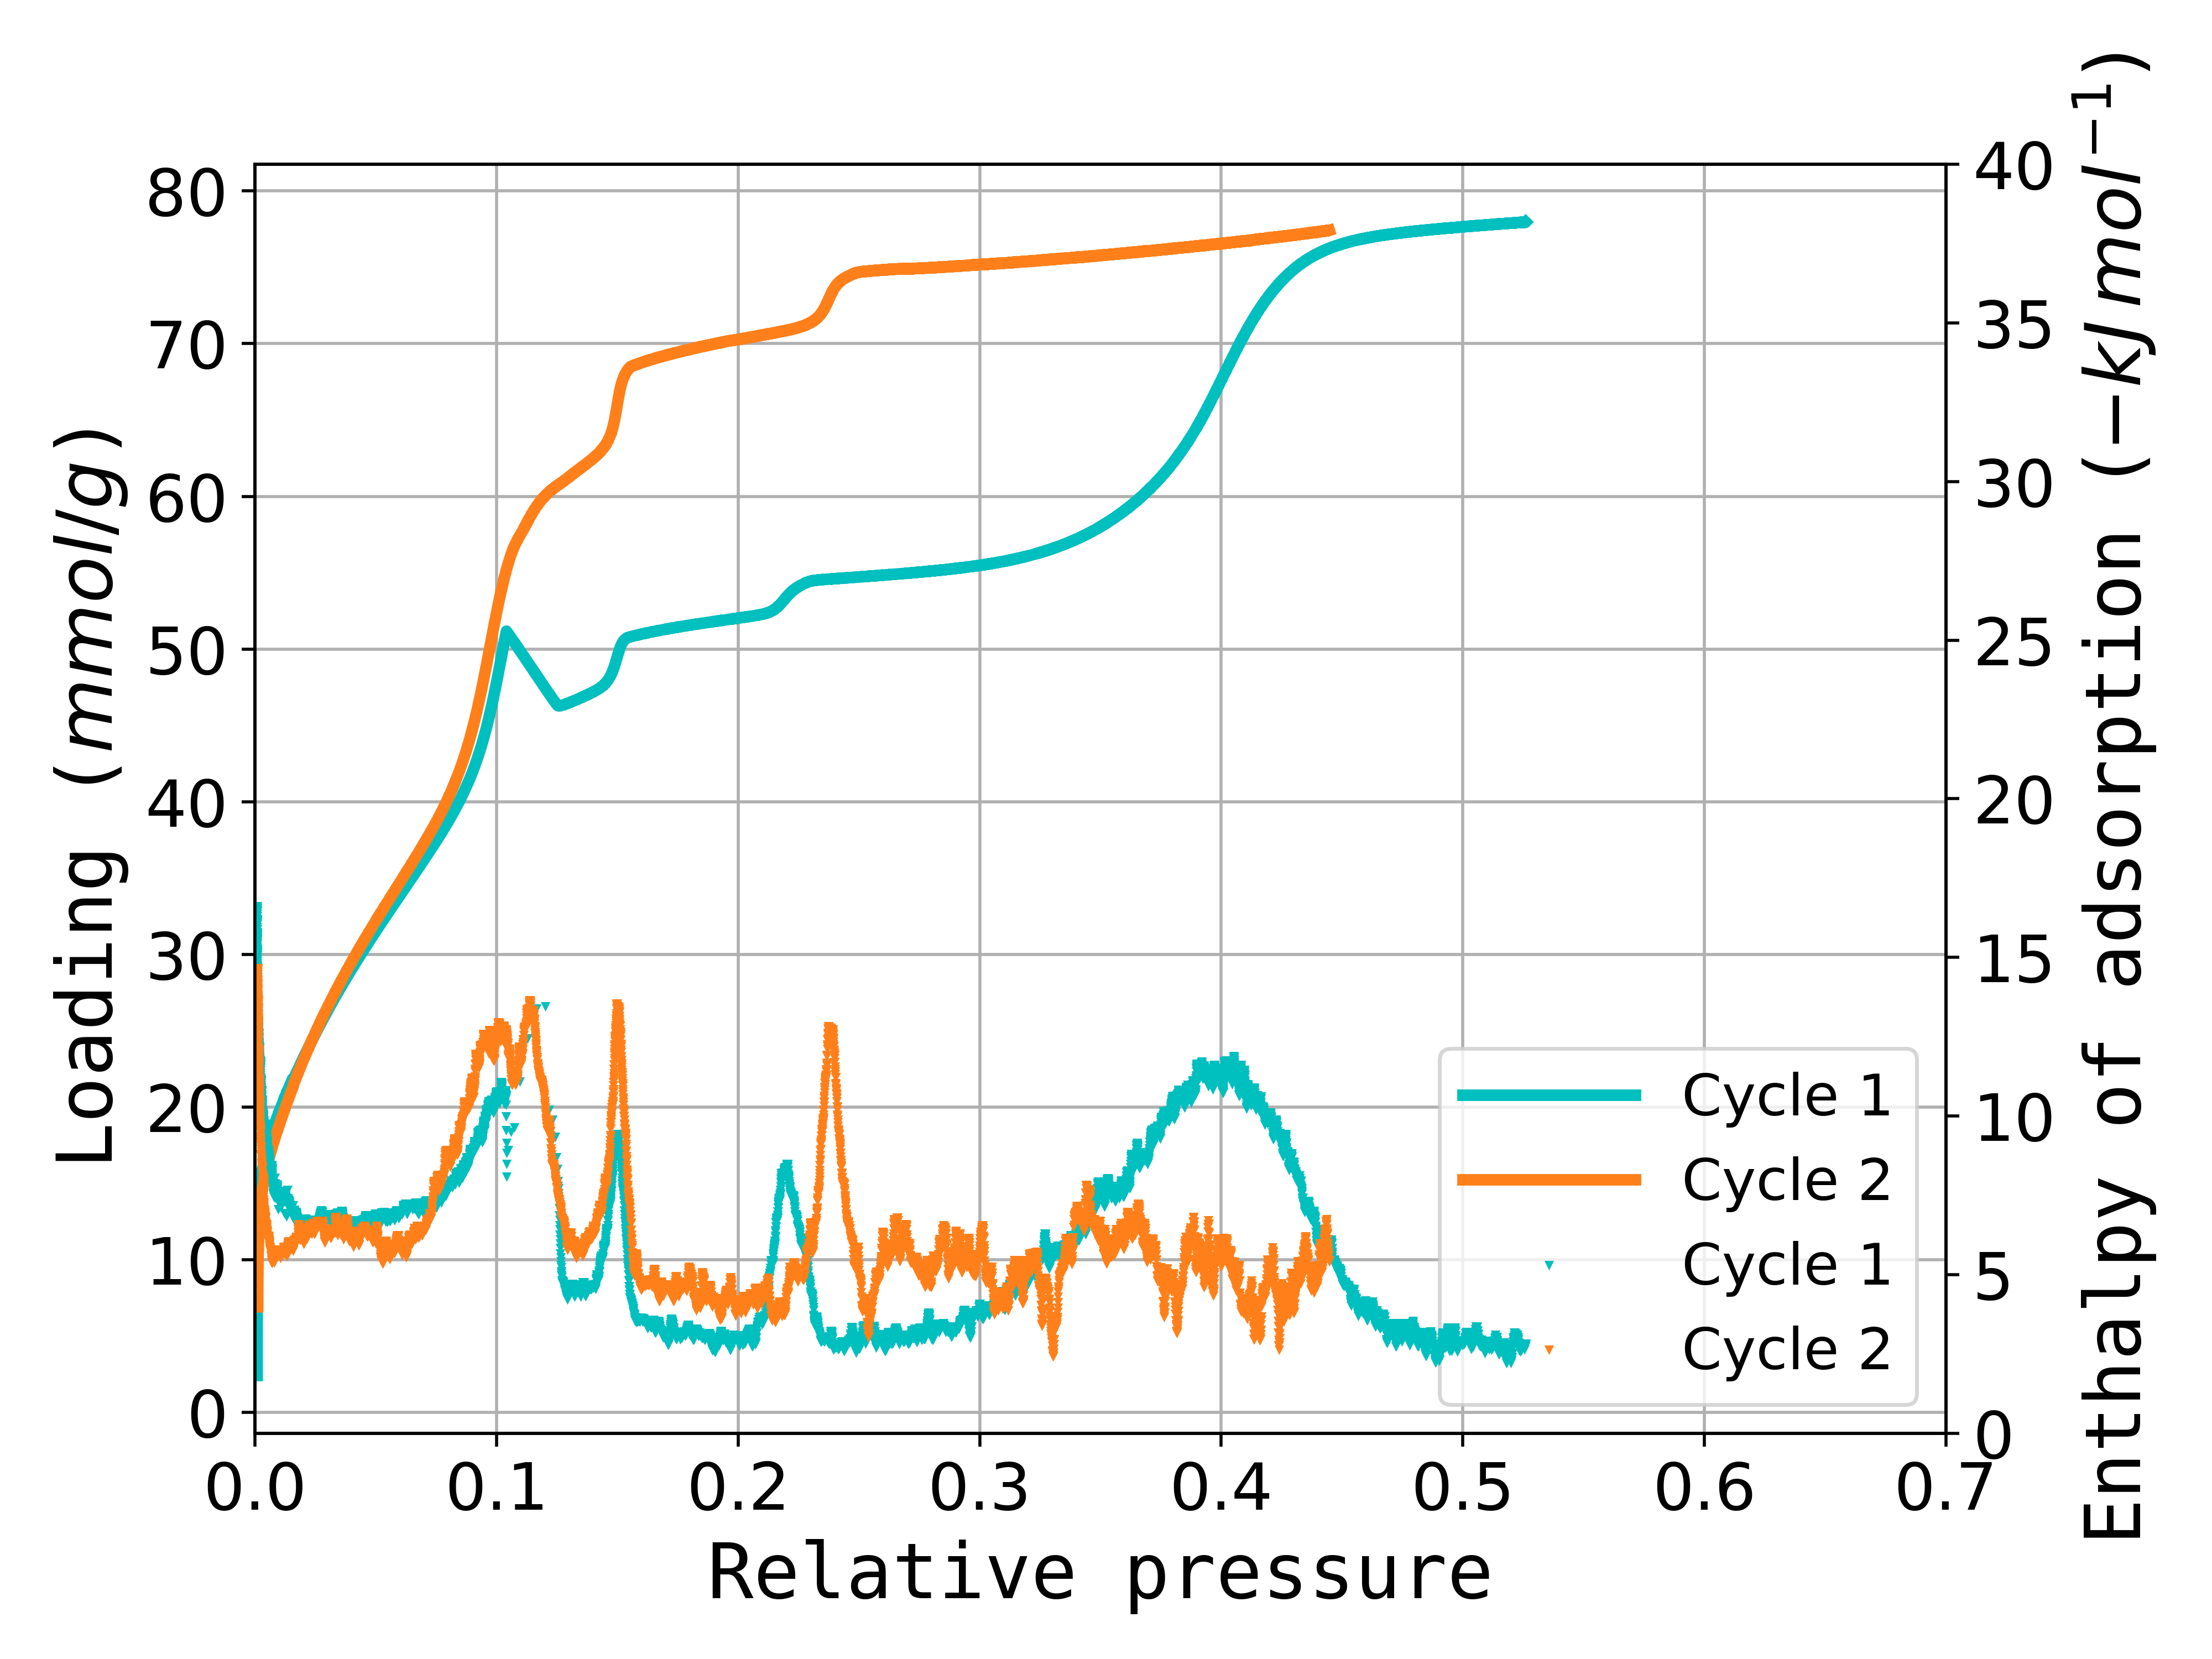
\includegraphics[width=\linewidth]{ltc/DUT-49-N2-cycled-reg}%
        \caption{}\label{dut:fgr:dut-49-cycle-reg}
    \end{subfigure}%
    \begin{subfigure}[h]{0.5\linewidth}
        \centering
        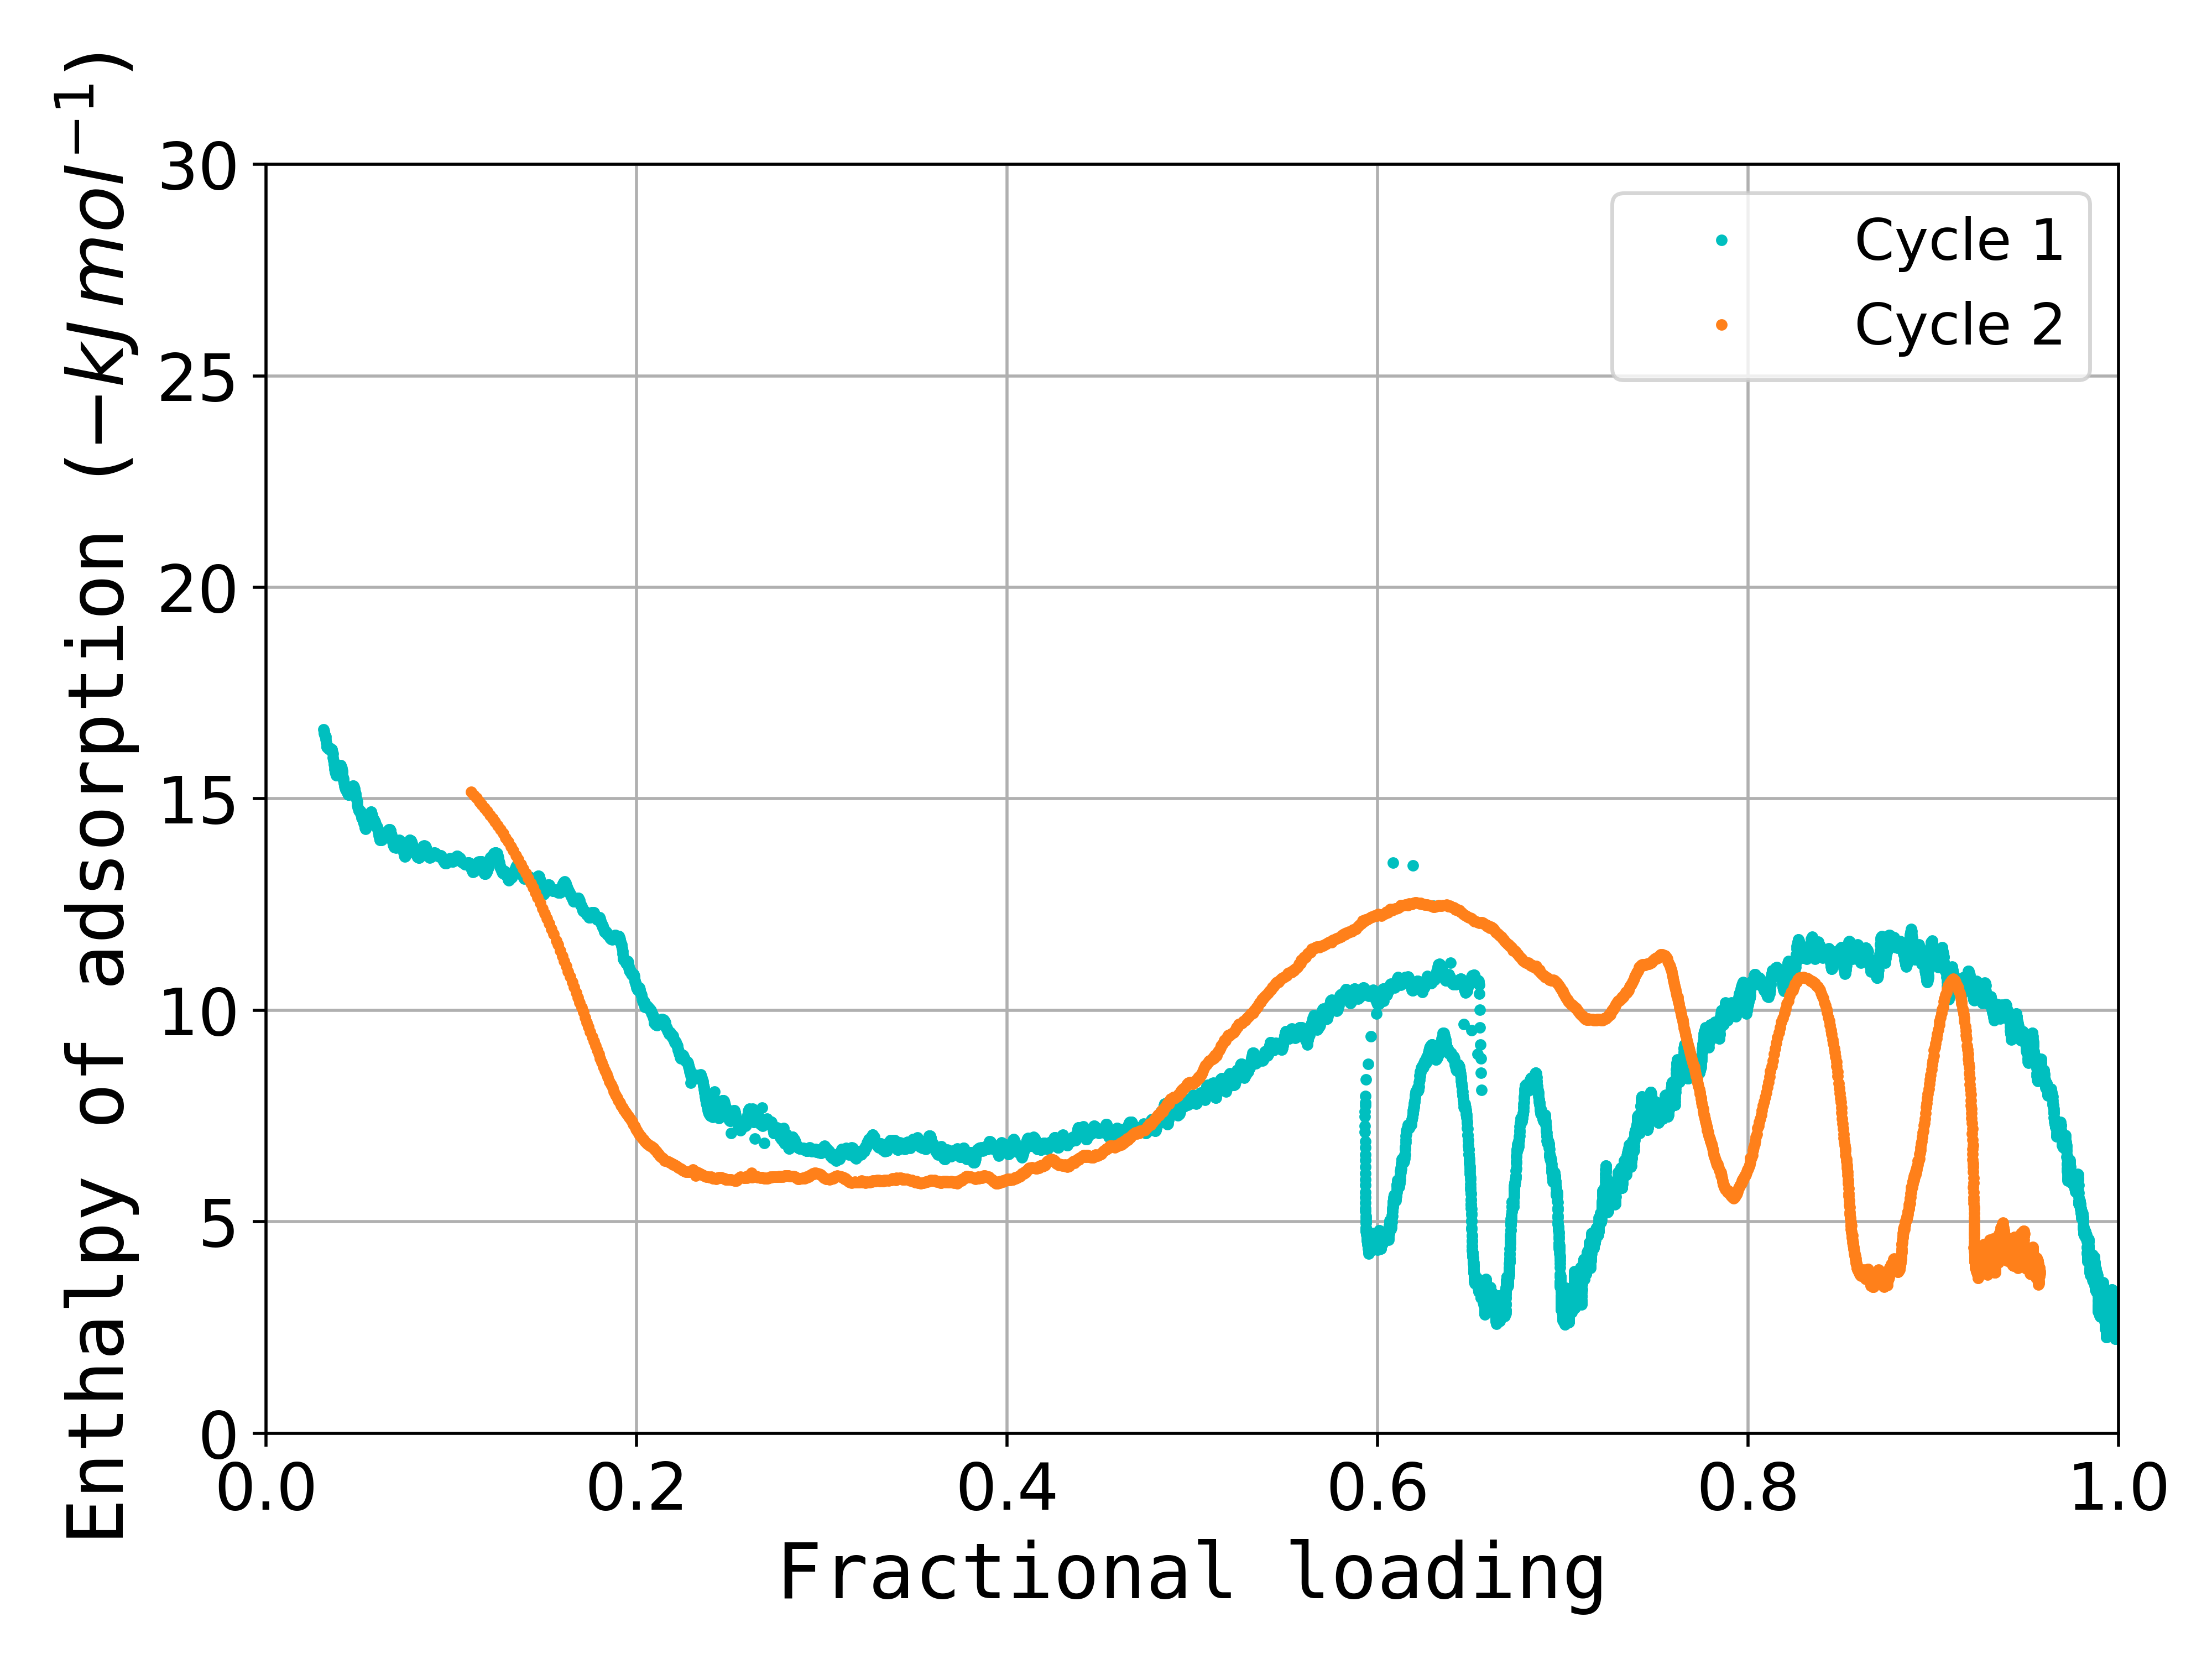
\includegraphics[width=\linewidth]{ltc/DUT-49-N2-cycled-enth}%
        \caption{}\label{dut:fgr:dut-49-cycle-enth}
    \end{subfigure}%
    \caption{Isotherms (a) and (b) enthalpy curves of nitrogen on
    cycled DUT-49. The first cycle is in black and the second 
    cycle is in blue.}%
    \label{dut:fgr:dut-49-cycle}
\end{figure}

Repeating nitrogen adsorption on a DUT-49 sample which has been
cycled in this manner reveals a different kind of isotherm, 
as seen in \autoref{dut:fgr:dut-49-cycle}. While the initial 
part of the isotherms is fully overlapped,
the second experiment does not have an NGA step. 
A structural transition still occurs, 
signalled by the small peak in the enthalpy curve at the end of the 
peak corresponding to the filling of the medium pore. However, instead
of a sudden contraction, the transition becomes a continuous 
process. The two progressive smaller re-opening steps still exist,
at similar partial pressure and with comparable differential enthalpy
of adsorption. Further cycling of this cell has shown only isotherms
of this kind. This effect is not seen on cycling with other 
adsorbents, with the NGA transition fully developed in each cycle. 

A possible explanation can be found if recalling the effect 
of crystal size on nitrogen induced 
NGA~\cite{krauseEffectCrystalliteSize2018}. It is likely 
that the sample exists as a mixture of different crystallite
sizes, some large enough to be capable of an NGA-type transition 
while smaller ones only contract to an intermediate pore state
(or even remain in the \textit{op} state).
The cycling may introduce large scale defects such as dislocations
or grain boundaries, effectively reducing the average crystal size
and increasing the percentage of material which cannot undergo 
complete contraction. 
Experimental evidence for the coexistence of both the \textit{cp} and 
\textit{op} phases after the transition pressure can be found in the 
\ce{^{129}Xe} NMR study performed 
by \citet{schaberSituMonitoringUnique2017}. In their paper,
the chemical shift of \ce{^{129}Xe} is monitored during
adsorption at \SI{200}{\kelvin}. The resulting peaks can be attributed
to the two phases of the material and a small
open pore signal is seen to be present concomitantly with the 
closed pore form.
This kind of behaviour further stresses the 
contribution of surface potentials on the occurrence of NGA.

\subsubsection{Overview of the mechanism of contraction in DUT-49}

From a structural perspective, two requirements are 
highlighted for NGA to occur.
First, the free energy surface as a function of loading and 
unit cell volume must have two local minima, corresponding to the 
two phases of the framework. An inversion of the overall stability
of the two phases must occur as the guest is loaded, which will 
place the system in a metastable state. While the transition
is energetically favoured, the activation barrier between the 
two forms must be overcome, and the contraction becomes 
kinetically controlled. The stability of the two phases 
depends on the combined contribution of the framework together
with the stabilisation effect of the adsorbed molecules,
which can also be represented as the
difference in \textit{integral} enthalpy of adsorption between the 
\textit{op} and \textit{cp} states. On the other hand, the 
energy barrier between the two states can be traced to the 
buckling limit of the linker.
